\chapter{Unit Test}
I følgende afsnit beskrives de unit test der bliver lavet. Der bruges Nunit\cite{NUnit}, som er en testing framework til vores testing af klasser. 

Diverse klasser vil blive testet i Testklassen af følgende syntaks "\big[Klasse\big]Unit". Methoderne skrevet i test klassen er skrevet med henblik over at det skal være lidt læseligt, og er opsat med følgende syntaks: 
\big[Hvad der testes\big]\_[I hvilke slags senarier]\_\big[og den forventet resultat\big] 

\section{Validator}
Validator-klassen er en statisk klasse, som har ansvar for at håndtere validering af input felterne i applikationen fra brugeren. For eksempel kan det være når brugeren skal indtaste sin Email.
\begin{figure}[H]
	\centering
	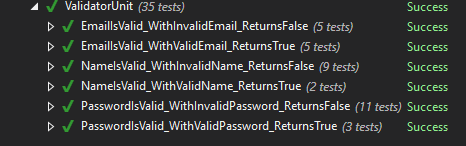
\includegraphics[width=0.6\linewidth]{Unit/ValidatorUnit.PNG}
	\caption{Screenshot af test sessionen på ValidatorUnit}
	\label{fig:ValidatorUnit}
\end{figure}
På figur \ref{fig:ValidatorUnit} ses følgende test der bliver udført. 